\section{Глава 1. Периодические решения уравнения Мэки-Гласса}

\begin{frame}
	\frametitle{Глава 1. Уравнение Мэки--Гласса}
	\begin{empheq}[box=\myeq]{equation}
		\label{eq:mg}
		\dot{x}=-\beta+\alpha\frac{e^{x(t-1)-x}}{1+e^{\gamma x(t-1)}}, \text{ где } \alpha, \beta > 0, \ \gamma \gg 1. \tag{MG}
	\end{empheq}

\end{frame}

\begin{frame}
	\frametitle{Релейное уравнение Мэки--Гласса}
	\small
	\begin{empheq}[box=\diseq]{equation*}
		\dot{x}=-\beta+\alpha\frac{e^{x(t-1)-x}}{1+e^{\gamma x(t-1)}}, \text{ где } \alpha, \beta > 0, \ \gamma \gg 1,
	\end{empheq}
	%
	\begin{empheq}[box=\myeq]{equation}
		\label{eq:mg_relay}
		\dot{x}=-\beta + \alpha e^{-x}F(\exp(x(t-1))), \text{ где } \alpha, \beta > 0, \ \gamma \gg 1, \tag{MGR}
	\end{empheq}
	%
	\begin{wrapfigure}{r}{0.4\textwidth} 
		\centering
		\includegraphics[width=0.5\textwidth]{F_relay_plot_intro.eps}
	\end{wrapfigure}
	%
	\begin{empheq}[box=\myeq]{equation*}
		F(u)=\lim\limits_{\gamma\to +\infty}\frac{u}{1+u^{\gamma}} = 
		\begin{cases}
			u, & 0 \leqslant u < 1;\\
			1/2, & u = 1;\\
			0, & u > 1.
		\end{cases}
	\end{empheq}
	\normalsize
	
\end{frame}

\begin{frame}
	\frametitle{Решение релейного уравнения}
	Введём обозначения:
	\begin{empheq}[box=\myeq]{equation*}
		T = \frac{1}{\beta} \ln\left(\frac{1}{2}\alpha^2e^{2\beta}(t_1 - 2)^2 + \alpha e^{\beta}(t_1 - 1) + 1\right),
	\end{empheq}
	где $t = t_1$ --- корень уравнения 
	\begin{empheq}[box=\myeq]{equation*}
		-\beta(t - 1) + \ln(\alpha e^{\beta}(t - 2) + 1) = 0,
	\end{empheq}
	\begin{empheq}[box=\myeq]{equation*}
		t_2 = 1 + T.
	\end{empheq}
\end{frame}

\begin{frame}
\frametitle{Решение релейного уравнения}
Определим множество начальных функций.

Зафиксируем положительные параметры $\sigma_0 < 1/2$, $p$, $q$ такие, что 
%
\begin{empheq}[box=\myeq]{equation*}
0 < p < \beta \sigma_0 < q.
\end{empheq}

Множество начальных функций:
%
\small
\begin{empheq}[box=\myeq]{multline*}
	S = \{\varphi\in C[-1 - \sigma_0, -\sigma_0]: 0 < p \leqslant \varphi(t)\leqslant q \\\text{ при } t \in [-1 - \sigma_0, -\sigma_0], \varphi(-\sigma_0) = \beta \sigma_0 \}.
\end{empheq}
\normalsize
%
\begin{center}
	\vspace{-6pt}
	\includegraphics[width=0.5\textwidth]{initial_func_S.eps}
\end{center}

\end{frame}

\begin{frame}
	\frametitle{Решение релейного уравнения}
	
	\textbf{Теорема} (О решении релейного уравнения).
	
	Пусть параметры $\alpha, \beta > 0$ удовлетворяют условиям
	%
	\footnotesize
	\begin{empheq}[box=\myeq]{equation*}
			\alpha > e^{\beta} - e^{-\beta} \text{ или } \alpha < \beta e^{\beta}, \quad 
			\frac{\alpha}{\beta}e^{\beta}\left(1 + \ln\frac{\beta}{\alpha}\right) < 1, \quad 
			\alpha > \dfrac{e^{\beta t_1} - 1}{e^{\beta}(t_1 - 1)}.
	\end{empheq}
	\normalsize
	Тогда релейное уравнение Мэки~--~Гласса \eqref{eq:mg_relay} с начальной функцией из множества $S$ имеет $T$-периодическое решение
	\small
	\begin{empheq}[box=\myeq]{equation*}
		x^*(t)= 
		\begin{cases}
				-\beta t, & t\in[-\sigma_0, 1],\\
				-\beta t +\ln(\alpha e^{\beta}(t - 1)+1), & t\in[1, 2],\\
				-\beta t + \ln(\frac{\alpha^2}{2}e^{2\beta}(t - 2)^2+\alpha e^{\beta}(t - 1)+1), & t\in[2, t_1],\\
				-\beta t + \ln(\frac{\alpha^2}{2}e^{2\beta}(t_1 - 2)^2+\alpha e^{\beta}(t_1 - 1) + 1), & t\in[t_1, t_2].
			\end{cases}
	\end{empheq}
	\normalsize
\end{frame}

\begin{frame}
	\frametitle{Решение релейного уравнения}
	%
	\footnotesize
	\begin{empheq}[box=\myeq]{equation*}
		x^*(t)= 
		\begin{cases}
			-\beta t, & t\in[-\sigma_0, 1],\\
			-\beta t +\ln(\alpha e^{\beta}(t - 1)+1), & t\in[1, 2],\\
			-\beta t + \ln(\frac{\alpha^2}{2}e^{2\beta}(t - 2)^2+\alpha e^{\beta}(t - 1)+1), & t\in[2, t_1],\\
			-\beta t + \ln(\frac{\alpha^2}{2}e^{2\beta}(t_1 - 2)^2+\alpha e^{\beta}(t_1 - 1) + 1), & t\in[t_1, t_2].
		\end{cases}
	\end{empheq}
	\normalsize
	\begin{center}
		\includegraphics[width=0.65\textwidth]{mg_relay.eps}
	\end{center}
	
\end{frame}

\begin{frame}
	\frametitle{Решение релейного уравнения}
	
	\textbf{Замечание.} Для выполнения условий
	%
	\footnotesize
	\begin{empheq}[box=\myeq]{equation*}
		\alpha > e^{\beta} - e^{-\beta} \text{ или } \alpha < \beta e^{\beta}, \quad 
		\frac{\alpha}{\beta}e^{\beta}\left(1 + \ln\frac{\beta}{\alpha}\right) < 1, \quad 
		\alpha > \dfrac{e^{\beta t_1} - 1}{e^{\beta}(t_1 - 1)}
	\end{empheq}
	\normalsize
	%
	достаточно
	\begin{empheq}[box=\myeq]{equation*}
		\beta > 0, \quad \alpha > \exp(\beta(1 + e^{-\beta})).
	\end{empheq}
	
\end{frame}

\begin{frame}
	\frametitle{Асимптотика решения}
	
	\footnotesize
	Пусть $\delta = \gamma^{-\nu}$ --- малый параметр, $\nu \in (\nicefrac{1}{2}, 1)$ --- константа.
	%
	Вне окрестностей точек излома $t_0$ и $t_1$ ищем решение в виде
	\begin{empheq}[box=\myeq]{equation*}
	x^*_\gamma(t, \varphi) = x^*(t) + \Delta(t, \varphi).
	\end{empheq}
	
	При $t \in [t_i - \delta, t_i + \delta]$, $i = 0, 1$, ищем решение в виде
	\begin{empheq}[box=\myeq]{gather*}
	x^*_\gamma(t, \varphi) = x^*(t_i) + \frac{1}{\gamma} w_i(\tau)|_{\tau = \gamma(t - t_i)} + \Delta(t, \varphi).\\
	w_i(\tau) = -\beta \tau - \dfrac{\alpha e^{-x^*(t_i)}}{\dot{x}^*(t_i - 1)} \ln\left(e^{-\dot{x}^*(t_i - 1)\tau} + 1\right) \, \text{при} \, \dot{x}^*(t_i - 1) > 0,\\
	w_i(\tau) = (-\beta + \alpha e^{-x^*(t_i)})\tau - \dfrac{\alpha e^{-x^*(t_i)}}{\dot{x}^*(t_i - 1)} \ln\left(e^{\dot{x}^*(t_i - 1)\tau} + 1\right) \, \text{при} \, \dot{x}^*(t_i - 1) < 0.
	\end{empheq}
	
	В обоих случаях доказываем малость остатка $\Delta(t, \varphi) = O(\gamma^{-2\nu})$.
	\normalsize
\end{frame}


\begin{frame}
	\frametitle{Асимптотические свойства функций $w_i(\tau)$}
	Верны следующие асимптотические равенства.
	
	\medskip
	
	Если $\dot{x}^*(t_i - 1) < 0$,
	\begin{empheq}[box=\myeq]{gather*}
		w_i(\tau) = -\beta \tau + O(\exp(-\dot{x}^*(t_i - 1) \tau)) \text{ при } \tau \to -\infty,\\
		w_i(\tau) = (-\beta + \alpha e^{-x^*(t_i)})\tau + O(\exp(\dot{x}^*(t_i - 1) \tau)) \text{ при } \tau \to +\infty,
	\end{empheq}
	
	Если $\dot{x}^*(t_i - 1) > 0$,
	\begin{empheq}[box=\myeq]{gather*}
		w_i(\tau) = (-\beta + \alpha e^{-x^*(t_i)})\tau + O(\exp(\dot{x}^*(t_i - 1) \tau)) \text{ при } \tau \to -\infty,\\
		w_i(\tau) = -\beta \tau + O(\exp(-\dot{x}^*(t_i - 1) \tau)) \text{ при } \tau \to +\infty.
	\end{empheq}
\end{frame}

\begin{frame}
	\frametitle{Асимптотика решения}
	\small
	\textbf{Теорема.} Пусть $\delta = \gamma^{-\nu}$, $\nu \in (\nicefrac{1}{2}, 1)$. Уравнение \eqref{eq:mg} с начальной функцией $\varphi \in S$ при соответствующих ограничениях на параметры $\alpha, \beta$ имеет решение $x_\gamma^*(t, \varphi)$ с асимптотикой
	\tiny
	\begin{empheq}[box=\myeq]{gather*}
		\label{eq:sol_x*gamma}
		x^*_\gamma(t, \varphi)= 
		\begin{cases}
			- \beta t + O(\gamma^{-1} e^{-\beta \delta \gamma}), & t\in[-\sigma_0, 1 - \delta],\\
			-\beta + \frac{1}{\gamma} w_0(\tau)|_{\tau=(t - 1)\gamma} + O(\gamma^{-2\nu}), & t \in [1 - \delta,1 + \delta]\\
			- \beta t + \ln(\alpha e^{\beta}(t - 1) + 1) + O(\gamma^{-2\nu}) & t\in[1 + \delta, 2]\\
			- \beta t + \ln(\frac{\alpha^2}{2}e^{2 \beta}(t - 2)^2 + \alpha e^{\beta}(t - 1) + 1) + O(\gamma^{-2\nu}) & t \in [2, t_1 - \delta]\\
			- \beta t_1 + \ln(\eta)+\frac{1}{\gamma} w_1(\tau)|_{\tau=(t - t_1)\gamma} + O(\gamma^{-2\nu}) & t\in[t_1 - \delta, t_1  +\delta]\\
			- \beta t + \ln(\eta) + O(\gamma^{-2\nu}) & t \in [t_1 + \delta, t_2 - \delta]
		\end{cases}
	\end{empheq}
	\small
	где $\eta=\frac{\alpha^2}{2}e^{2\beta}(t_1 - 2)^2 + \alpha e^{\beta}(t_1 - 1) + 1$.
	
	Асимптотические выражения приведены при $\gamma\to+\infty$.
	
	Все остатки равномерны по $\varphi$ и $t$ из соответствующих промежутков.
	\normalsize
\end{frame}

%
%\begin{frame}
%	\frametitle{Вычисление асимптотики}
%	Пусть
%	$$\delta = \gamma^{-\nu}, \quad \nu \in (1/2, 1).$$
%	%
%	Вне окрестностей точек излома $t_0$ и $t_1$ ищем решение в виде
%	\[
%	x^*_\gamma(t, \varphi) = x^*(t) + \Delta(t, \varphi).
%	\]
%	
%	При $t \in [t_i - \delta, t_i + \delta]$ ищем решение в виде
%	\[
%	x^*_\gamma(t, \varphi) = x^*(t_i) + \frac{1}{\gamma} w_i(\tau)|_{\tau = \gamma(t - t_i)} + \Delta(t, \varphi).
%	\]
%	%
%    \[
%    w_i(\tau) = -\beta \tau - \dfrac{\alpha e^{-x^*(t_i)}}{\dot{x}^*(t_i - 1)} \ln\left(e^{-\dot{x}^*(t_i - 1)\tau} + 1\right) \, \text{при} \, \dot{x}^*(t_i - 1) > 0,
%    \]
%    \[
%    w_i(\tau) = (-\beta + \alpha e^{-x^*(t_i)})\tau - \dfrac{\alpha e^{-x^*(t_i)}}{\dot{x}^*(t_i - 1)} \ln\left(e^{\dot{x}^*(t_i - 1)\tau} + 1\right) \, \text{при} \, \dot{x}^*(t_i - 1) < 0,
%    \]
%\end{frame}

\begin{frame}
	\frametitle{Существование периодического решения}
	
	\begin{empheq}[box=\myeq]{equation*}
		\Pi_{\gamma}: S(\sigma_0, p, q) \to S(\sigma_0, p, q)
	\end{empheq}
	%
	\begin{empheq}[box=\myeq]{equation*}
		\Pi_{\gamma}(\varphi(t)) = x^*_{\gamma}(t + T_{\gamma, \varphi}, \varphi), \quad t\in[-1-\sigma_0, -\sigma_0].
	\end{empheq}
	
	\begin{center}
		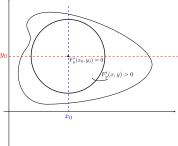
\includegraphics[width=0.6\linewidth]{mg_poincare.eps}
	\end{center}
\end{frame}

\begin{frame}
	\frametitle{Основная теорема}
	
	\textbf{Теорема.} Пусть параметры $\alpha > 0$, $\beta > 0$ удовлетворяют условиям
	%
	\footnotesize
	\begin{empheq}[box=\myeq]{equation*}
		\alpha > e^{\beta} - e^{-\beta} \text{ или } \alpha < \beta e^{\beta}, \quad 
		\frac{\alpha}{\beta}e^{\beta}\left(1 + \ln\frac{\beta}{\alpha}\right) < 1, \quad 
		\alpha > \dfrac{e^{\beta t_1} - 1}{e^{\beta}(t_1 - 1)}.
	\end{empheq}
	\normalsize
	Тогда для произвольной начальной функции $\varphi \in S$ и достаточно больших $\gamma$ уравнение Мэки~--~Гласса \eqref{eq:mg} имеет решение $x^*_\gamma(t, \varphi)$ периода $T_{\gamma, \varphi}$, причём
	
	\small
	\begin{empheq}[box=\myeq]{equation*}
		\lim\limits_{\gamma \to +\infty} \max\limits_{t \in [-\sigma_0, T_{\gamma, \varphi} - \sigma_0]} |x^*_\gamma(t, \varphi) - x^*(t)| = 0,
	\end{empheq}
	
	\begin{empheq}[box=\myeq]{equation*}
		\lim\limits_{\gamma \to +\infty} T_{\gamma, \varphi} = T.
	\end{empheq}
	\normalsize
	
	Пределы равномерны по $\varphi \in S$.
	
\end{frame}

\section{Глава 2. Дискретные бегущие волны в полносвязной сети релейных генераторов Мэки--Гласса}


\begin{frame}
	\frametitle{Глава 2. Полносвязная цепь генераторов Мэки--Гласса}
	
	Полносвязная сеть из $(N + 1)$ релейных генераторов Мэки--Гласса:
	
	\begin{empheq}[box=\myeq]{equation*}
		\dot{u}_j(t) = -\beta u_j(t) + \alpha F \bigg(u_j(t - 1) + \sum\limits_{k = 0, k\neq j}^N u_k(t)\bigg), \quad j = 0, 1, \dots, N.
	\end{empheq}
	
	\begin{figure}
		\centering
		\includegraphics[width=0.5\textwidth]{full_mesh_u.eps}
	\end{figure}
\end{frame}


\begin{frame}
	\frametitle{Дискретная бегущая волна}
	
	\begin{empheq}[box=\myeq]{equation*}
		u_j(t) = u(t - j\Delta),\quad j = 0, 1, \ldots, N, \text{ где } \Delta > 0 \text{ --- сдвиг.}
	\end{empheq}
	
	Если $u\left(t - (N + 1)\Delta\right) = u(t)$, после подстановки в систему все уравнения обращаются в уравнение с $N$ запаздываниями
	
	\begin{empheq}[box=\myeq]{equation*}
		\label{eq:mg_aux1}
		\dot{u} = -\beta u + \alpha F\left(u(t - 1) + \sum_{s=1}^{N} u(t - s\Delta)\right). \tag{AUX}
	\end{empheq}
	
	Уравнение периодов:
	
	\begin{empheq}[box=\myeq]{equation*}
		pT(\Delta) = (N + 1)\Delta \quad \text{при некотором } p \in \mathbb{N}.
	\end{empheq}
	
	
\end{frame}

\begin{frame}
	\frametitle{Решение вспомогательного уравнения}
	
	Множество начальных функций:
	\footnotesize
	\begin{empheq}[box=\myeq]{equation*}
		S_1 = \{\varphi \in C[-\tau, 0] \,|\, \varphi(t) > 0\}, \tau = \max\{N\Delta, 1\}.
	\end{empheq}
	\normalsize
	
	\footnotesize
	\textbf{Теорема}. Пусть $\alpha > \exp\left(\beta(1 + e^{-\beta})\right)$. Для произвольной положительной начальной функции из множества $S_1$ уравнение \eqref{eq:mg_aux1} имеет решение
	\begin{empheq}[box=\myeq]{equation*}
		u_*(t)=
		\begin{cases}
			u_0 e^{-\beta t}(\alpha A(t-t_0)+1) & \text{ при } t\in[t_0,t_0+1],
			\\
			u_0 e^{-\beta t}\left(\frac{\alpha^2}{2}Ae^{\beta}(t-t_0-1)^2+\alpha A(t-t_0)+1\right) & \text{ при } t\in[t_0+1,t_1],
			\\
			u_0 e^{-\beta t}\left(\frac{\alpha^2}{2}Ae^{\beta}(t_1-t_0-1)^2+\alpha A(t_1-t_0)+1\right) & \text{ при } t\in[t_1,t_0+T],
		\end{cases}
	\end{empheq}
	\normalsize
	%
	\[
	u_*(t+T)\equiv u_*(t),
	\]
	
	Здесь $A = e + e^{\Delta} + e^{2\Delta} + \ldots + e^{N\Delta}$, $t_0$, $t_1$ --- точки переключения.
\end{frame}

\begin{frame}
	\frametitle{Решение вспомогательного уравнения}

\footnotesize
	\begin{empheq}[box=\myeq]{equation*}
		u_*(t)=
		\begin{cases}
			u_0 e^{-\beta t}(\alpha A(t-t_0)+1) & \text{ при } t\in[t_0,t_0+1],
			\\
			u_0 e^{-\beta t}\left(\frac{\alpha^2}{2}Ae^{\beta}(t-t_0-1)^2+\alpha A(t-t_0)+1\right) & \text{ при } t\in[t_0+1,t_1],
			\\
			u_0 e^{-\beta t}\left(\frac{\alpha^2}{2}Ae^{\beta}(t_1-t_0-1)^2+\alpha A(t_1-t_0)+1\right) & \text{ при } t\in[t_1,t_0+T],
		\end{cases}
	\end{empheq}
\normalsize
	
	\begin{center}
		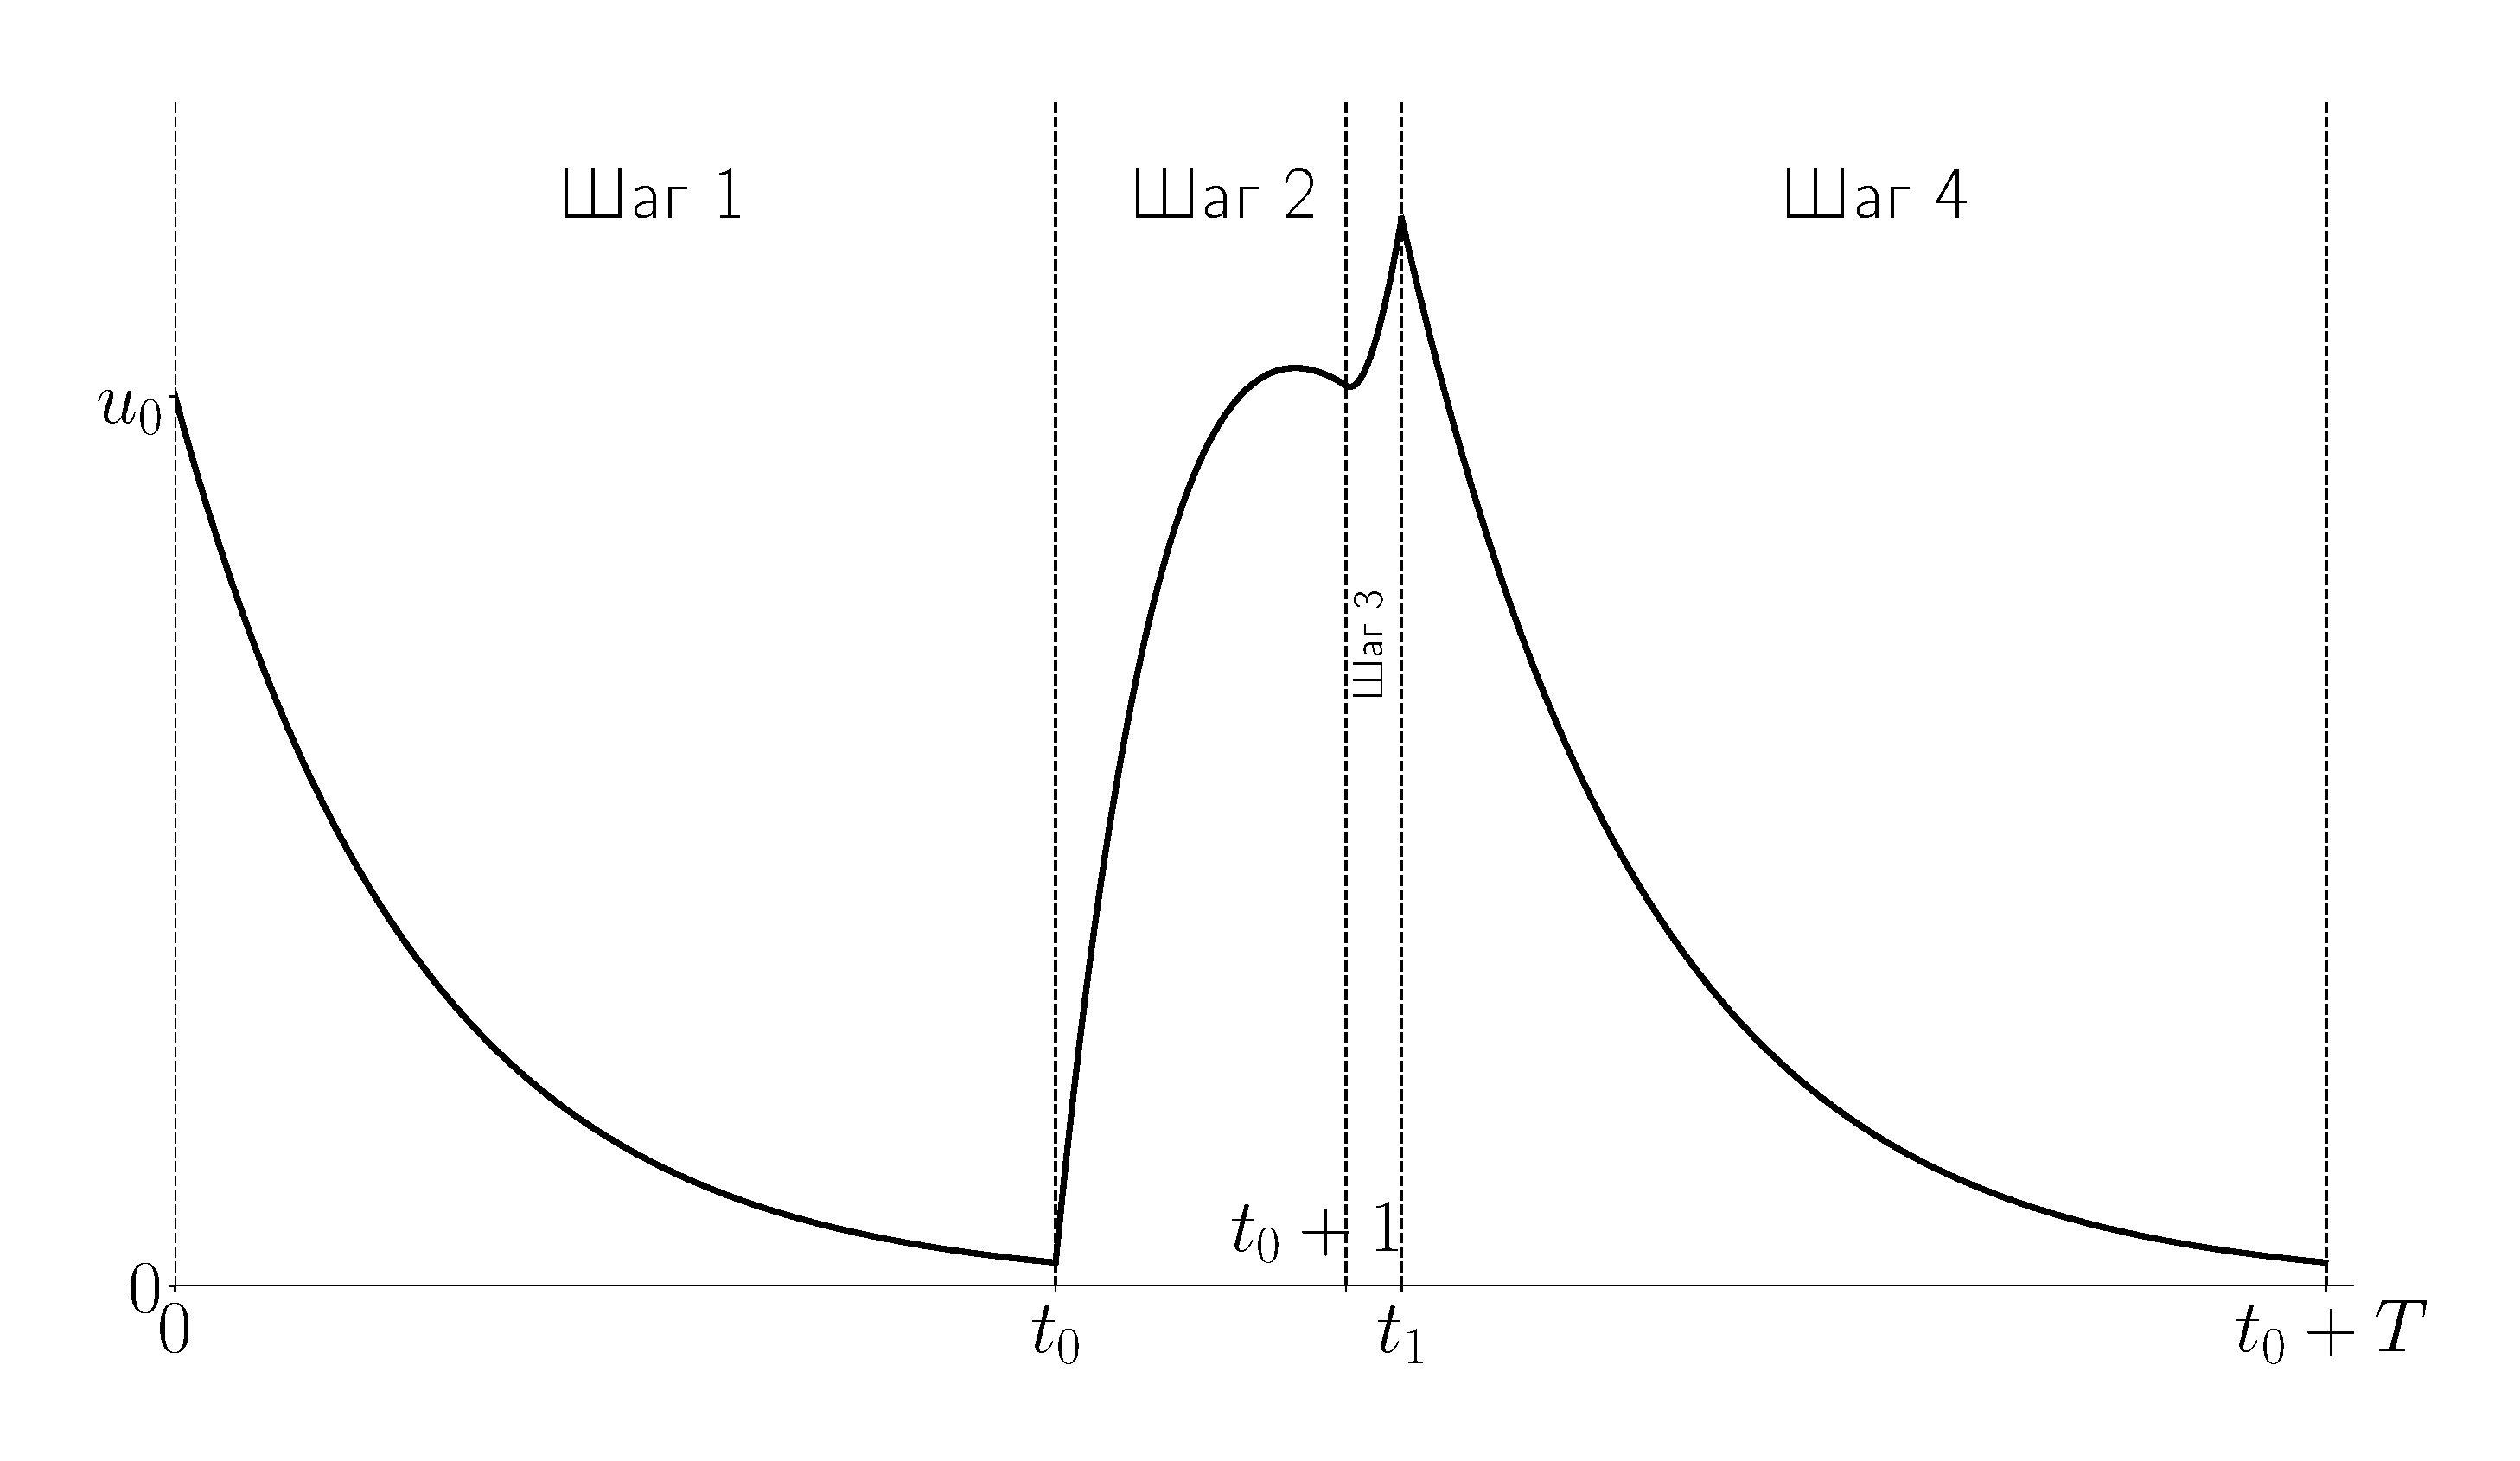
\includegraphics[width=0.8\textwidth]{u_star.eps}
	\end{center}
\end{frame}

\begin{frame}
	\frametitle{Бегущая волна: теорема существования}
	
	\textbf{Теорема.} 
	Для произвольных $\beta > 0$, $\alpha > \exp\left(\beta(1 + e^{-\beta})\right)$
	существует единственное значение $\Delta > 1$, при котором 
	\begin{enumerate}
		\item вспомогательное уравнение с параметрами $\alpha, \beta, \Delta$ имеет $T$-периодическое решение $u_*(t)$, причём $T = (N + 1) \Delta$;
		\item соответствующий набор функций
		\[u_j(t) = u_*(t + j \Delta), j = 0, \ldots N\]
		(с точностью до нумерации компонент) является решением в виде дискретной бегущей волны.
	\end{enumerate}
	
\end{frame}

\begin{frame}
	\frametitle{Бегущая волна: численные результаты}
	
	На рисунках показана независимость от выбора начальных функций:
	
	\begin{center}
		\includegraphics[width=0.8\linewidth]{a5p0_b1p2_N2_solution_start.eps}
		
		\includegraphics[width=0.8\linewidth]{a5p0_b1p2_N2_const_start.eps}
		
		\includegraphics[width=0.8\linewidth]{a5p0_b1p2_N2_random_start.eps}
	\end{center}
\end{frame}

\section{Глава 3. Режимы двухкластерной синхронизации в полносвязной сети релейных генераторов Мэки-Гласса}

\begin{frame}
	\frametitle{Глава 3. Двухластерная синхронизация}
	
	Полносвязная сеть из $N = m + n$ генераторов Мэки~--~Гласса описывается системой	
	\begin{empheq}[box=\myeq]{equation*}
		\dot{u}_j(t) = -\beta u_j(t) + \alpha F_{\gamma} \bigg(u_j(t - 1) + \delta\sum\limits_{k = 0, k\neq j}^N u_k(t)\bigg), \quad j = 0, 1, \dots, N.
	\end{empheq}
	
	\begin{wrapfigure}{r}{0.4\textwidth} 
		\vspace{-23pt} 
		\centering
		\includegraphics[width=0.5\textwidth]{two_cluster_uv.eps}
	\end{wrapfigure}
	
	Периодическое решение системы вида
	\begin{empheq}[box=\myeq]{multline*}
		u_1(t)=\ldots=u_m(t) = u(t),\\u_{m+1}(t)=\ldots=u_{m+n}(t) = v(t)
	\end{empheq}
	называется режимом двухкластерной синхронизации.
	
\end{frame}

\begin{frame}
	\frametitle{Вспомогательная система}
	\small
	После подстановки 
	$$u_1(t)=\ldots=u_m(t) = u(t), \, u_{m+1}(t)=\ldots=u_{m+n}(t) = v(t)$$
	получаем вспомогательную систему:
	\begin{empheq}[box=\myeq]{equation*}
		\label{eq:pres:aux}
		\begin{cases}
			\dot{u} = -\beta u + \alpha \, F_{\gamma} \big(u(t - 1) + \delta (m - 1) u + \delta n v\big),\\
			\dot{v} = -\beta v + \alpha \, F_{\gamma} \big(v(t - 1) + \delta m u + \delta (n - 1) v\big).
		\end{cases}\tag{AUX2}
	\end{empheq}
	
	Произведём замену 
	\begin{empheq}[box=\myeq]{equation}
	\label{eq:pres:tilde_change}
		\begin{cases}
			\tilde{u}(t) = u(t - 1) + \delta (m - 1) u + \delta n v,\\ \tilde{v}(t) = v(t - 1) + \delta m u + \delta (n - 1) v.
		\end{cases}
	\end{empheq}
	
	\textbf{Теорема 1.} Замена \eqref{eq:pres:tilde_change} обратима в классе $T$-периодических непрерывно дифференцируемых функций ($T > 0$).
	\normalsize
	
\end{frame}

\begin{frame}
	\frametitle{Двухкластерная синхронизация в полносвязной сети}
	
	После замены система примет вид
	%
	\small
	\begin{empheq}[box=\myeq]{equation}
		\label{eq:pres:mg_cluster_system_tilde}
		\begin{cases}
			\dot{\tilde{u}} = -\beta \tilde{u} + \alpha \big(F_{\gamma}(\tilde{u}(t - 1)) + \delta (m - 1) \, F_{\gamma}(\tilde{u}) + \delta n \, F_{\gamma}(\tilde{v})\big),\\
			\dot{\tilde{v}} = -\beta \tilde{v} + \alpha \big(F_{\gamma}(\tilde{v}(t - 1)) + \delta m \, F_{\gamma}(\tilde{u}) + \delta (n - 1) \, F_{\gamma}(\tilde{v})\big).
		\end{cases}
	\end{empheq}
	\normalsize
	
	
	\textbf{Теорема 2.} Если неотрицательные $T$-периодические функции $\tilde{u}, \tilde{v}$ являются решением системы \eqref{eq:pres:mg_cluster_system_tilde}, то выраженные из соотношений \eqref{eq:pres:tilde_change} функции $u, v$ являются решением вспомогательной системы \eqref{eq:pres:aux}.
\end{frame}

\begin{frame}{Экспоненциальная замена}
	
	После экспоненциальной замены
	\begin{empheq}[box=\myeq]{equation*}
		\tilde{u} = e^x, \quad \tilde{v} = e^y
	\end{empheq}
	и ввода функции 
	\begin{empheq}[box=\myeq]{equation*}
		G_{\gamma}(x) = e^{-x} \, F_{\gamma} (e^x) = \dfrac{1}{1 + e^{\gamma x}},
	\end{empheq}
	получаем итоговый вид системы:
	\footnotesize
	\begin{empheq}[box=\myeq]{equation*}
		\begin{cases}
			\dot{x} = -\beta + \alpha \left(e^{x(t - 1) - x} G_{\gamma}(x(t - 1)) + \delta (m - 1) G_{\gamma}(x) + \delta n e^{y - x} G_{\gamma}(y)\right),\\
			\dot{y} = -\beta + \alpha \left(e^{y(t - 1) - y} G_{\gamma}(y(t - 1)) + \delta m e^{x - y} G_{\gamma}(x) + \delta (n - 1) G_{\gamma}(y)\right).
		\end{cases}
	\end{empheq}
	\normalsize
\end{frame}

\begin{frame}{Переход к релейной системе}
	Пусть 
	\begin{empheq}[box=\myeq]{equation*}
		G(x) = \lim\limits_{\gamma \to +\infty} G_{\gamma}(x) = \lim\limits_{\gamma \to +\infty} \dfrac{1}{1 + e^{\gamma x}} = \begin{cases}
			1, & x < 0;\\
			1/2, & x = 0;\\
			0, & x > 0.
		\end{cases}
	\end{empheq}
	
	Перейдём к релейной системе
	\footnotesize
	\begin{empheq}[box=\myeq]{equation*}
		\begin{cases}
			\dot{x} = -\beta + \alpha \left(e^{x(t - 1) - x} G(x(t - 1)) + \delta (m - 1) G(x) + \delta n e^{y - x} G(y)\right),\\
			\dot{y} = -\beta + \alpha \left(e^{y(t - 1) - y} G(y(t - 1)) + \delta m e^{x - y} G(x) + \delta (n - 1) G(y)\right).
		\end{cases}
	\end{empheq}
	\normalsize
	
	Множество начальных функций:
	\footnotesize
	\begin{empheq}[box=\myeq]{equation*}
		S_2 = \{(\varphi, \psi) \in (C[-1, 0])^2 \,|\, \varphi(t) > 0, \psi(t) > 0, x_0 = \varphi(0), y_0 = \psi(0), x_0 > y_0 \}.
	\end{empheq}
	\normalsize
\end{frame}
%
%\begin{frame}{Первый шаг решения системы}
%	
%	Пусть $\alpha > \frac{\beta}{\delta (n - 1)}$. Решение продолжается только вдоль прямой $y = 0$. Тогда $G(0) = \frac{\beta}{\delta(n - 1)} = \frac{1}{2}$?
%	
%	\begin{center}
%		\includegraphics[width=\textwidth]{cluster_1_step.png}
%	\end{center}
%\end{frame}

\begin{frame}{Обобщённое решение уравнения}
	Релейная система не имеет решения при $t > \frac{y_0}{\beta}$. Ищем решение в обобщённом смысле. Введём предстоящие определению функции $g_x(x, t)$, $g_y(y, t)$; перепишем систему в виде:
	\footnotesize
	\begin{empheq}[box=\myeq]{equation*}
		\begin{cases}
			\dot{x} = -\beta + \alpha \left(e^{x(t - 1) - x} g_x(x(t - 1), t - 1) + \delta (m - 1) g_x(x, t) + \delta n e^{y - x} g_y(y, t)\right),\\
			\dot{y} = -\beta + \alpha \left(e^{y(t - 1) - y} g_y(y(t - 1), t - 1) + \delta m e^{x - y} g_x(x, t) + \delta (n - 1) g_y(y, t)\right),\\
			g_x(x, t) = G(x) \text{  при  } x \neq 0,\\
			g_y(y, t) = G(y) \text{  при  } y \neq 0. 
		\end{cases}
	\end{empheq}
	\normalsize
		
	Решение данной системы называется обобщённым решением релейной системы (в смысле Филиппова).
	
\end{frame}

\begin{frame}{Решение системы}
	\textbf{Теорема 3.} При ограничениях на параметры
	\footnotesize
	\begin{empheq}[box=\myeq]{gather*}
		\label{eq:constraint_2}
		\beta < \alpha \delta (m - 1), \quad \beta < \alpha \delta (n - 1),\\
		\label{eq:constraint_3}
		e^{\beta} \cdot \dfrac{n - \delta(n - 1)}{\delta (n - 1)^2} > \dfrac{1}{n - 1} + \dfrac{1}{\delta(m - 1)}, \quad
		e^{\beta} \cdot \dfrac{m - \delta(m - 1)}{\delta (m - 1)^2} > \dfrac{1}{\delta(n - 1)} + \dfrac{1}{m - 1}.
	\end{empheq}
	\normalsize
	релейная система с начальной функцией из множества $S_2$ имеет единственное (обобщённое) решение следующего вида
	\begin{center}
	% plot_step_by_step_solution, 2024-06-22 двухкластерная синхронизация XY.ipynb
	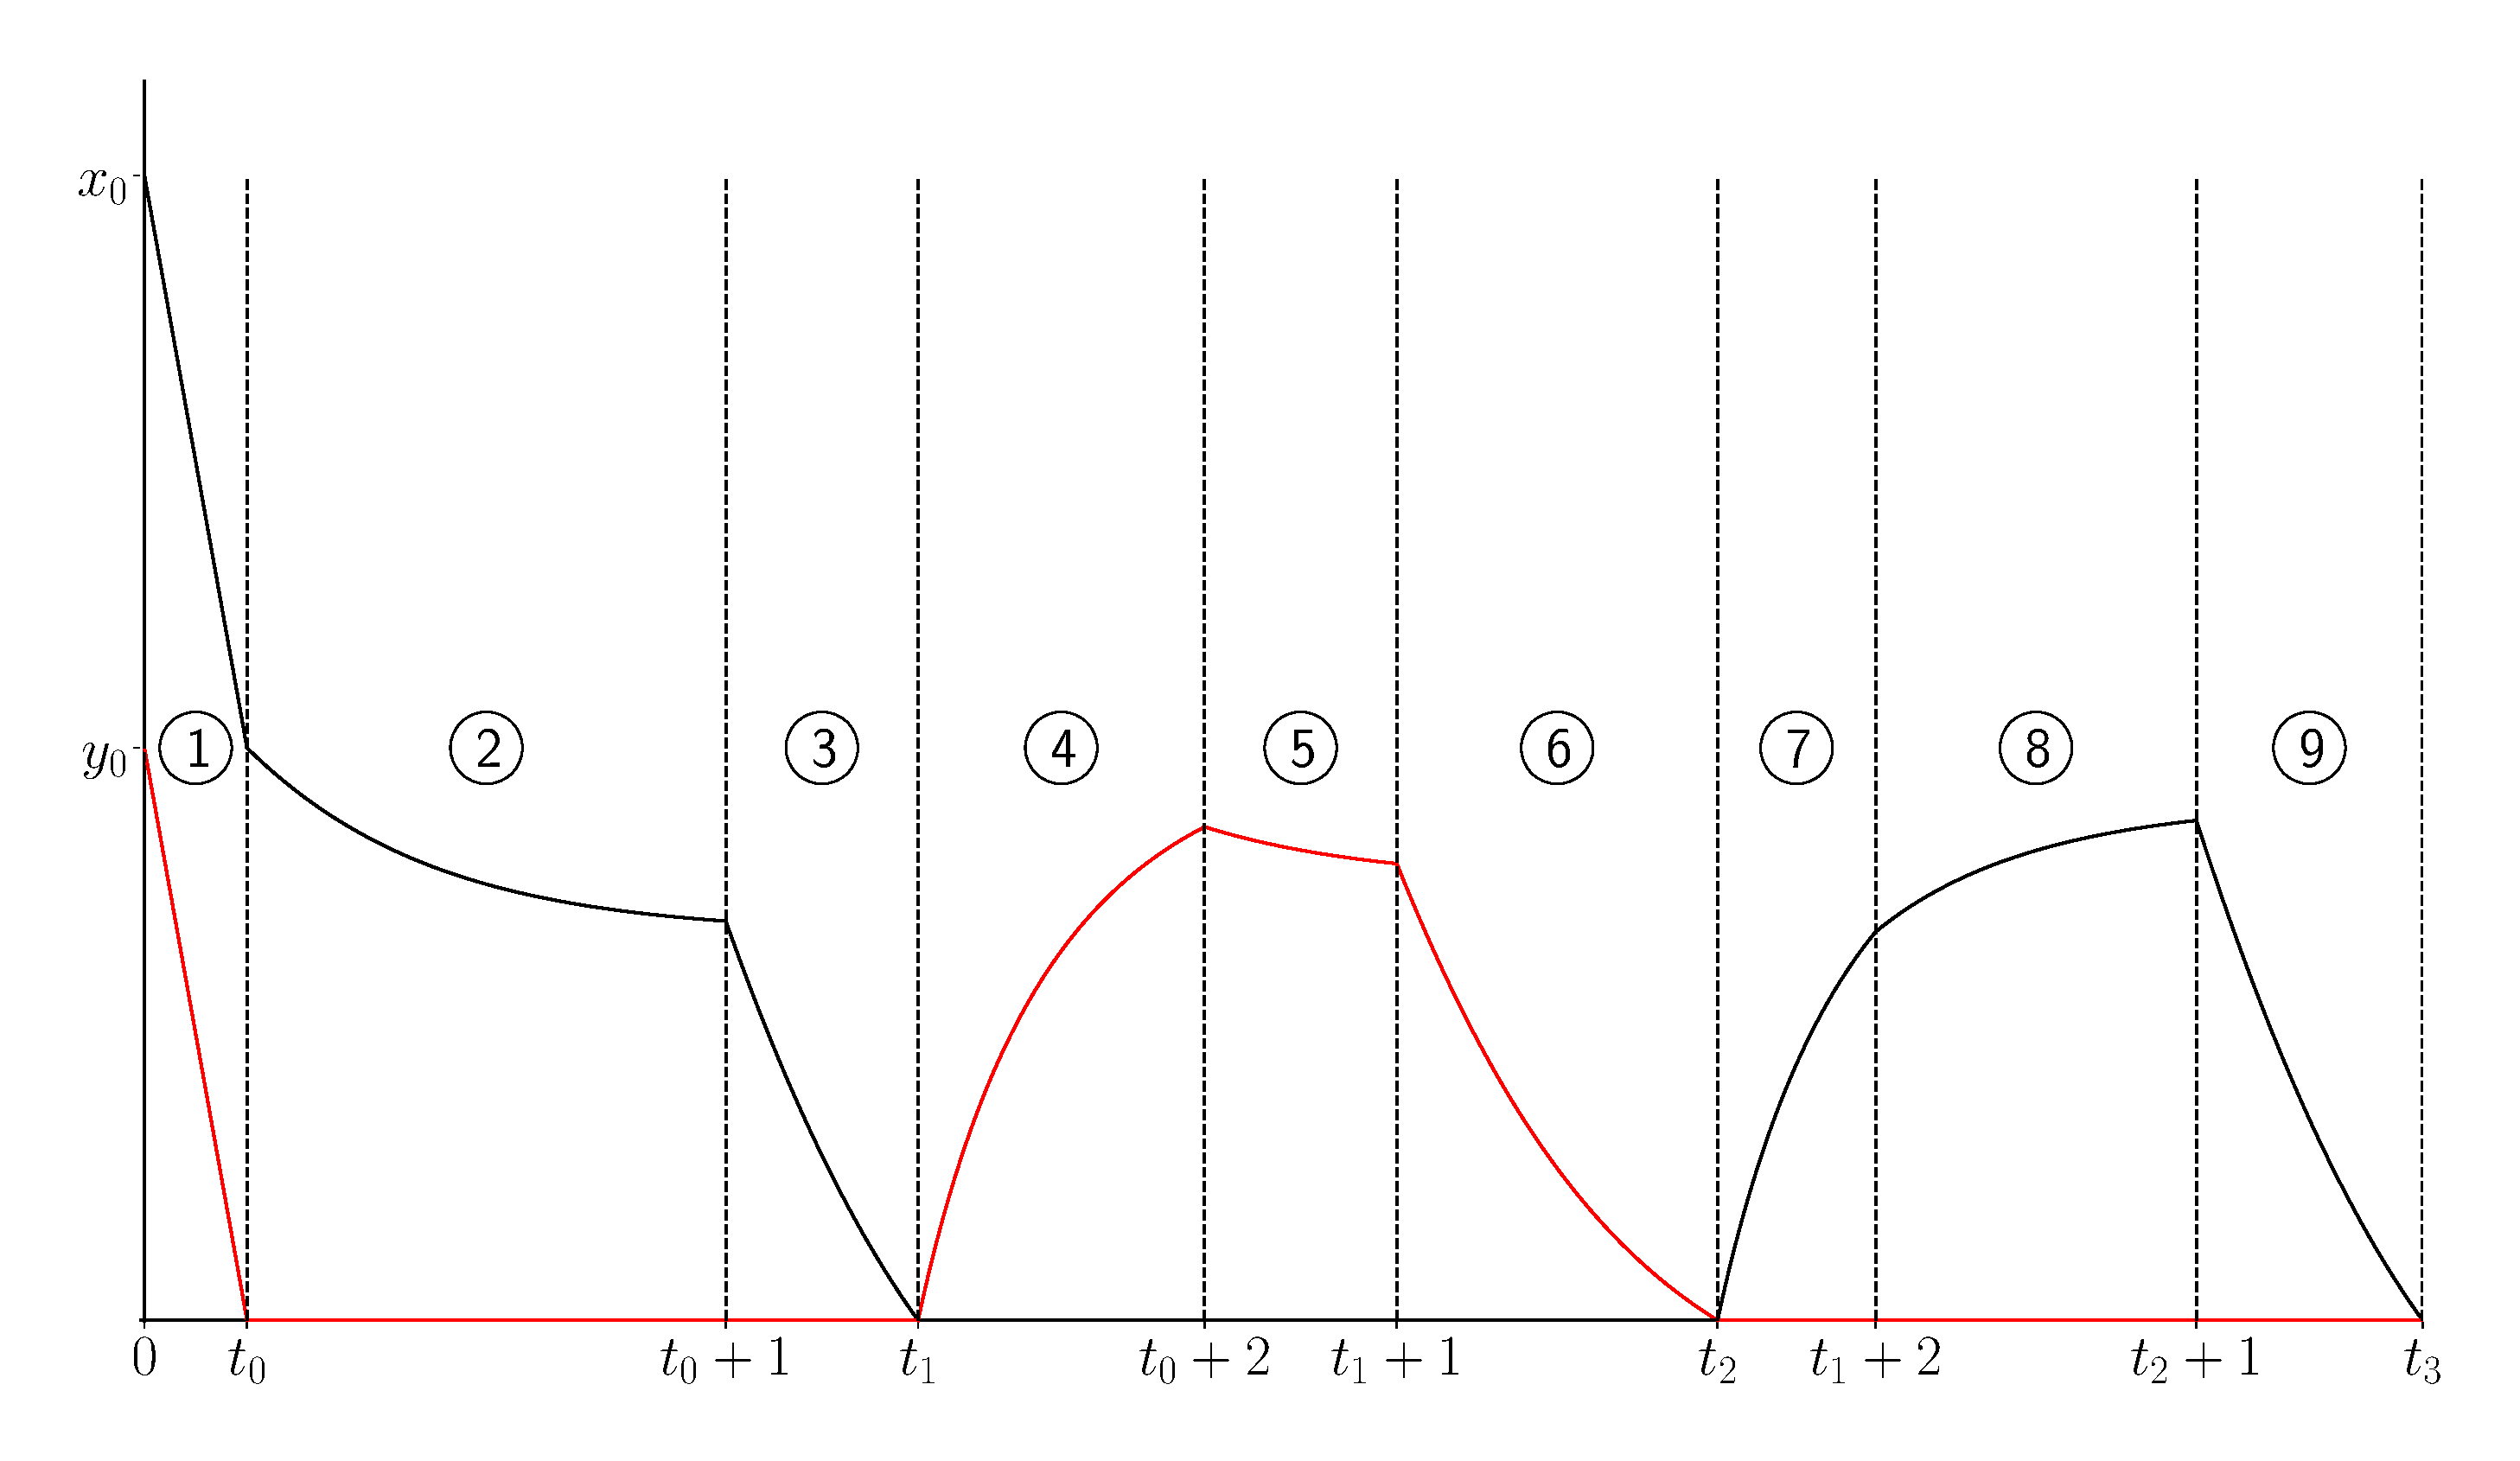
\includegraphics[width=0.7\linewidth]{cluster_step_by_step.eps}
	\end{center}
\end{frame}


\begin{frame}
	\frametitle{Основная теорема}
	\textbf{Теорема 4.} При ограничениях на параметры из теоремы 3, существует периодическое обобщённое решение $x(t)$, $y(t)$ релейной системы, соответствующее шагам 4 -- 9 решения, изображённого выше.
	
	\begin{center}
		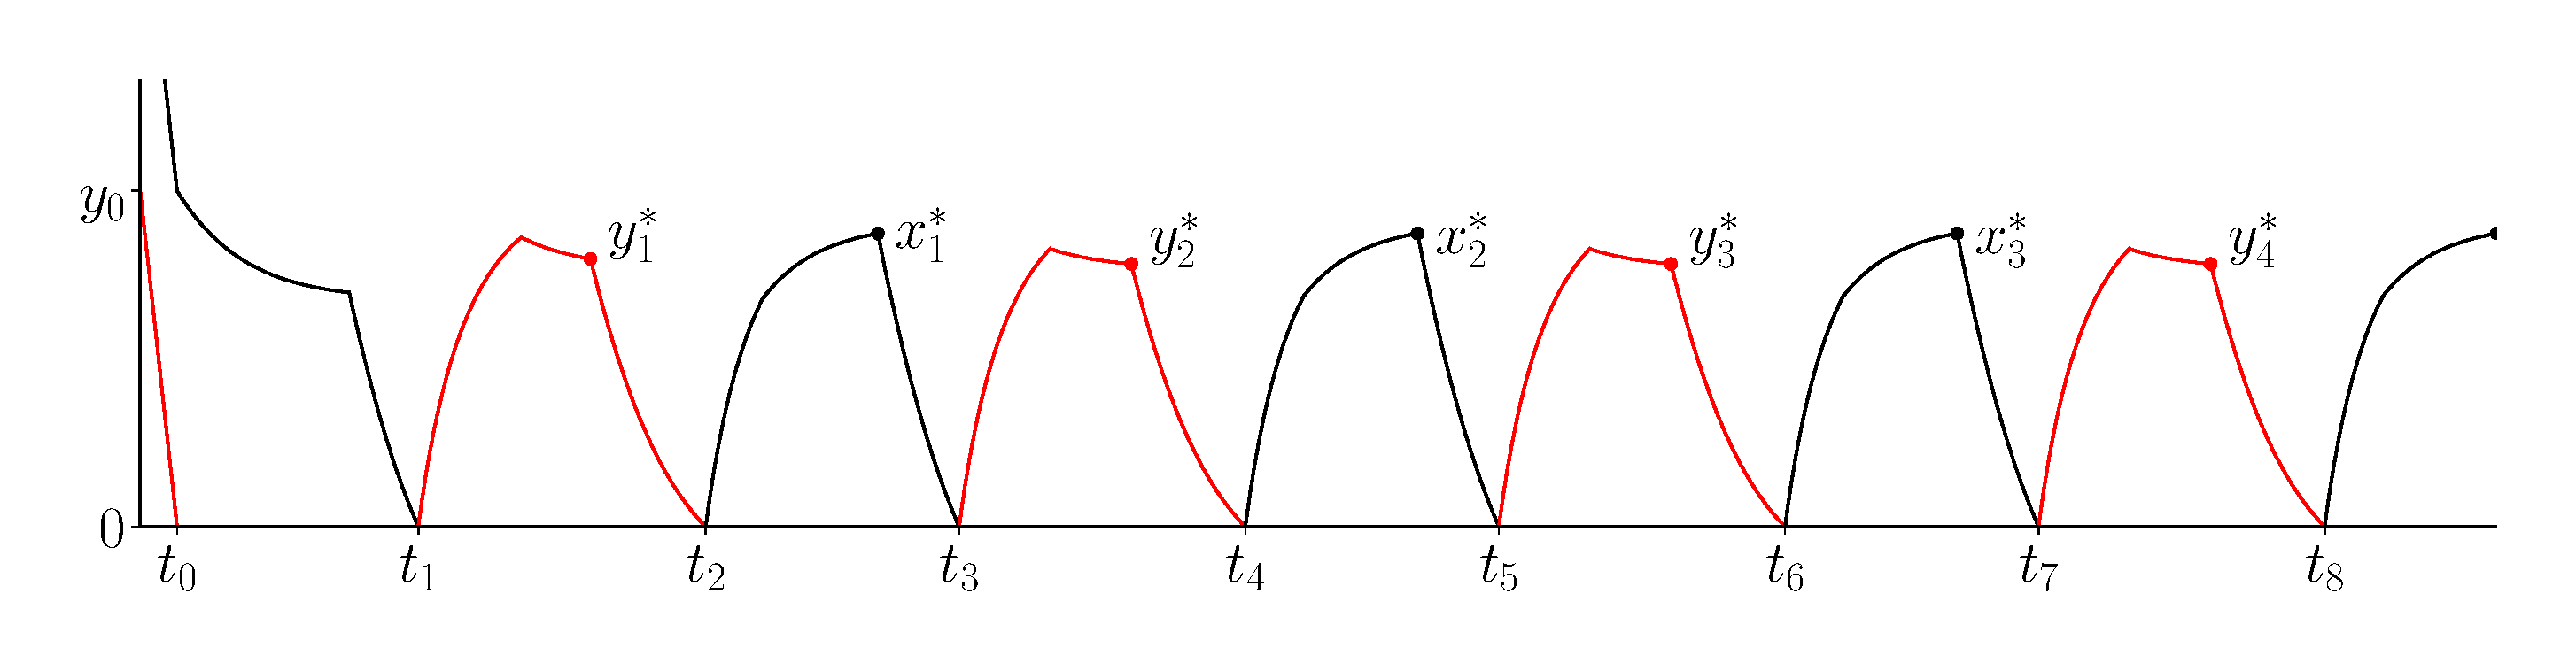
\includegraphics[width=\textwidth]{cluster_stars.eps}
	\end{center}
\end{frame}

\begin{frame}
	\frametitle{Численные результаты}
	
	Результаты численного моделирования.
	\includegraphics[height=1.2em]{ptr1.png} --- решение релейной системы, \includegraphics[height=1em]{ptr2.png}  --- решение системы при $\gamma = 200$, \includegraphics[height=1em]{ptr3.png} --- решение системы при $\gamma = 20$.
	
	% 2024-06-22 двухкластерная синхронизация XY 
	\begin{center}
	\includegraphics[width=0.8\linewidth]{cluster_solution_1.eps}
	
	\smallskip
	
	\includegraphics[width=0.8\linewidth]{cluster_solution_2.eps}
	\end{center}
\end{frame}
